% !TEX program=lualatex
\RequirePackage{luatex85}
\documentclass[10pt,tikz]{standalone}

\usepackage{luatextra} % also loads fixltx2e, fontspec, xunicode
\usepackage{microtype} % Slightly tweak font spacing for aesthetics
\usepackage{mathtools}
\usepackage{amsmath}
\usepackage{unicode-math}
\usepackage{xcolor}

\usepackage{tikz}
\usetikzlibrary{shapes,arrows,positioning,calc,decorations.pathmorphing}

\setmainfont{TeX Gyre Heros}
\setmathfont{Latin Modern Math}

\definecolor{colorR}{RGB}{228,26,28}    % RED
\definecolor{colorB}{RGB}{55,126,184}   % BLUE
\definecolor{colorG}{RGB}{77,175,74}    % GREEN
\definecolor{colorP}{RGB}{152,78,163}   % PURPLE
\definecolor{colorO}{RGB}{255,127,0}    % ORANGE
\definecolor{colorY}{RGB}{255,255,51}   % YELLOW
\definecolor{colorBn}{RGB}{166,86,40}   % BROWN
\definecolor{colorPk}{RGB}{247,129,191} % PINK
\definecolor{colorGy}{RGB}{153,153,153} % GRAY
\definecolor{maroon}{RGB}{140,29,64}

\tikzstyle{line}=[draw, -stealth', line width=0.8pt]
\tikzstyle{lab}=[font=\footnotesize,pos=0.5,inner sep=0.1pt,sloped,above=1.5mm]
\tikzstyle{ref}=[sep=0.1]

\begin{document}
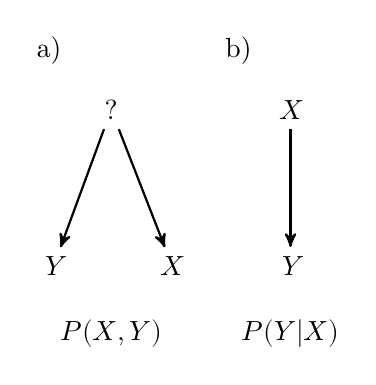
\begin{tikzpicture}[node distance=8mm, auto]

% pair-HMM
\node (?) {?};
\node[above left=2mm and 3mm of ?] {a)};
\node[below right=15mm and 3mm of ?] (X-pairhmm) {$X$};
\node[below left=15mm and 3mm of ?] (Y-pairhmm) {$Y$};
\path[line] (?) to (X-pairhmm);
\path[line] (?) to (Y-pairhmm);

\node[below=23mm of ?] {$P(X,Y)$};

% FST
\node[right=18mm of ?] (X-fst) {$X$};
\node[above left=2mm and 1mm of X-fst] {b)};
\node[below=15mm of X-fst] (Y-fst) {$Y$};
\path[line] (X-fst) to (Y-fst);

\node[below=23mm of X-fst] {$P(Y|X)$};

% % composition
% \node[right=10mm of X-fst] (X-comp) {$X$};
% \node[above left=2mm and 1mm of X-comp] {c)};
% \node[below=5mm of X-comp] (Y-comp) {$Y$};
% \node[below=5mm of Y-comp] (Z-comp) {$Z$};
% \path[line] (X-comp) to (Y-comp);
% \path[line] (Y-comp) to (Z-comp);
%
% \node[below=23mm of X-comp] {$P(Z|X)$};

\end{tikzpicture}
\end{document}
